%\documentclass[notes,11pt,aspectratio=169]{beamer}
\documentclass[11pt,aspectratio=169]{beamer}
\usetheme{auriga} %Themes http://www.hartwork.org/beamer-theme-matrix/
\usecolortheme{auriga}


\definecolor{red}{RGB}{255, 0, 0}
\definecolor{blue}{RGB}{0, 118, 186}
\definecolor{green}{RGB}{0,255,0}
\definecolor{gray}{RGB}{146, 146, 146}
\definecolor{colorA}{RGB}{96, 34, 59}
\definecolor{colorB}{RGB}{140, 151, 154}
\definecolor{secinhead}{RGB}{249,196,95}
\definecolor{titlebg}{RGB}{51,51,51}
%\setbeamercolor{structure}{fg=colorA,bg=colorB}
\setbeamercolor{secsubsec}{fg=secinhead,bg=black}
%\setbeamercolor{frametitle}{fg=secinhead,bg=red}
\setbeamercolor{block title}{fg=red}




%=================================================
% packages and new commands
%=================================================
\usepackage[ruled, linesnumbered, vlined]{algorithm2e}
\usepackage{multirow, algorithmic, amsmath}
\usepackage[french]{babel} % babel system, adjust the language of the content
\usepackage{animate}


\usepackage{pgfpages}
\usepackage{fancyvrb}
\usepackage{tikz}
\usepackage{pgfplots}
\usepackage{tikz}
\usetikzlibrary{trees}
\usetikzlibrary{arrows, decorations.markings}

\usetikzlibrary{shadows}

\usepackage{transparent,graphicx,xcolor}



\setbeamertemplate{note page}[plain]

%\setbeameroption{show notes}
%\setbeameroption{show notes on second screen=right}


%% Beamer pass-through options
\DeclareOptionBeamer{compress}{\beamer@compresstrue}
\DeclareOptionBeamer{deutsch}{\@uzhdeutschtrue}
\DeclareOptionBeamer{german}{\@uzhdeutschtrue}
\ProcessOptionsBeamer

%% Theme options
\DeclareOption{deutsch}{\@uzhdeutschtrue}
\DeclareOption{german}{\@uzhdeutschtrue}
\DeclareOption{informal}{\@uzhinformaltrue}
\DeclareOption{formal}{\@uzhinformalfalse}
\ProcessOptions


% fonts

\newcommand\importantstuff[3]{
	\node[black!30!white] at (#1+0.1,#2-0.1) {
		\scalebox{2}{\Huge\texttt{#3}} 
	};
	\node at (#1,#2) {
		\scalebox{2}{\Huge\texttt{#3}} 
	};
}

\RequirePackage{eulervm}% math font that blends better with Bookman
\setbeamerfont{title}{size={\fontsize{20}{24pt}\selectfont},parent=structure,series=\bfseries}
\setbeamerfont{subtitle}{size={\fontsize{9}{11pt}\selectfont},series=\mdseries}
\setbeamerfont{author}{size={\fontsize{9}{11pt}\selectfont},series=\mdseries}
\setbeamerfont{footline}{size={\fontsize{5}{7pt}\selectfont}}% originally also: shape=\itshape
\setbeamercolor{footline}{fg=black}
\setbeamerfont{frametitle}{parent=structure,size={\fontsize{12}{14pt}\selectfont},series=\bfseries}
\setbeamerfont{framesubtitle}{parent=frametitle,size=\footnotesize}
\setbeamerfont{uzhunit}{size={\fontsize{7}{9pt}\selectfont},series=\bfseries,family=\sffamily}




\tikzstyle{vecArrow} = [thick, decoration={markings,mark=at position
	1 with {\arrow[semithick]{open triangle 60}}},
double distance=1.4pt, shorten >= 5.5pt,
preaction = {decorate},
postaction = {draw,line width=1.4pt, white,shorten >= 4.5pt}]
\tikzstyle{innerWhite} = [semithick, white,line width=1.4pt, shorten >= 4.5pt]


\tikzstyle{every picture}+=[remember picture]

% By default all math in TikZ nodes are set in inline mode. Change this to
% displaystyle so that we don't get small fractions.
\everymath{\displaystyle}

\usetikzlibrary{calc,fadings}
\tikzfading[name=fade l,left color=transparent!100,right color=transparent!0]
\tikzfading[name=fade r,right color=transparent!100,left color=transparent!0]
\tikzfading[name=fade d,bottom color=transparent!100,top color=transparent!0]
\tikzfading[name=fade u,top color=transparent!100,bottom color=transparent!0]

% this "frames" a rectangle node
\newcommand\framenode[2][10pt]{
	\fill[white,path fading=fade u] (#2.south west) rectangle ($(#2.south east)+(0, #1)$);
	\fill[white,path fading=fade d] (#2.north west) rectangle ($(#2.north east)+(0,-#1)$);
	\fill[white,path fading=fade l] (#2.south east) rectangle ($(#2.north east)+(-#1,0)$);
	\fill[white,path fading=fade r] (#2.south west) rectangle ($(#2.north west)+( #1,0)$);
}

\makeatletter
\let\insertsupervisor\relax
\newcommand\supervisortitle{Sous la direction de}
\mode<all>
{
	\newcommand\supervisor[1]{\def\insertsupervisor{#1}}
	\titlegraphic{}
}
\defbeamertemplate*{title page}{supdefault}[1][]
{
	\vbox{}
	\vfill
	\begingroup
	\centering
	\begin{beamercolorbox}[sep=8pt,center,#1]{title}
		\usebeamerfont{title}\inserttitle\par%
		\ifx\insertsubtitle\@empty\relax%
		\else%
		\vskip0.25em%
		{\usebeamerfont{subtitle}\usebeamercolor[fg]{subtitle}\insertsubtitle\par}%
		\fi%     
	\end{beamercolorbox}%
	\vskip1em\par
	\begin{beamercolorbox}[sep=8pt,center,#1]{author}
		\usebeamerfont{author}\insertauthor
	\end{beamercolorbox}
	\ifx\insertsupervisor\relax\relax\else
	\begin{beamercolorbox}[sep=8pt,center,#1]{}
		\usebeamerfont{author}\supervisortitle:~\insertsupervisor
	\end{beamercolorbox}\fi
	\begin{beamercolorbox}[sep=8pt,center,#1]{institute}
		\usebeamerfont{institute}\insertinstitute
	\end{beamercolorbox}
	\begin{beamercolorbox}[sep=8pt,center,#1]{date}
		\usebeamerfont{date}\insertdate
	\end{beamercolorbox}\vskip0.5em
	
	{\usebeamercolor[fg]{titlegraphic}\inserttitlegraphic\par}
	\endgroup
	\vfill
}

\title[ \hspace{0.8cm} \insertframenumber/\inserttotalframenumber]{{\sc Interview for PhD position at CEA-ATLAS Saclay team }}


 
\author{{ Ismail EZZAKI}}


\newcommand*{\rom}[1]{\expandafter\@slowromancap\romannumeral #1@}




%=================================================
% start presentation
%=================================================
\begin{document}
	
	\setbeamertemplate{titlepage}[supdefault]

{
  % rather than use the frame options [noframenumbering,plain], we make the
  % color match, so that the indicated page numbers match PDF page numbers
  %\setbeamercolor{page number in head/foot}{fg=background canvas.bg}
  \begin{frame}
   \begin{center}	\includegraphics[width=0.9\linewidth,height=0.2\textheight]{figures/header.png}\\
  \end{center}
  
    \titlepage
  \end{frame}
}
\begin{frame}

  \frametitle{Plan
  }
	\tableofcontents
\end{frame}

%========================
% your slides:
%========================




\section{About me}
 
\begin{frame}{\underline{\secname}}
	
\begin{center}
\textbf{About me}
\end{center}

\begin{itemize}
	\item Ismail EZZAKI
	\item 22 years old
	\item From Morocco
	\item I’ve always been interested in discovering how things work
	\item Childhood dream: win Nobel prize in physics
	\item Realistic dream (age > 12 yrs) : be an academic researcher
\end{itemize}	


\end{frame}


\begin{frame}{\underline{\secname}}
	
	\begin{center}
		\textbf{Academic background}
	\end{center}
	\begin{columns}
		\begin{column}{0.5\linewidth}
	
	\begin{itemize} 			  \setlength\itemsep{0em}

		\item 2014: High School in Experimental sciences
		\item 2018: B.Sc. in Fundamental Physics
		
		\item 2020: M.Sc. in High energy physics and computational physics
	\end{itemize}	

			\end{column}
		
	\pause	
		\begin{column}{0.5\linewidth}
		
	\begin{itemize}			  \setlength\itemsep{0em}

		\item 2014: Programming
		\item 2018: Machine \& Deep learning
	\end{itemize}
			\end{column}
	\end{columns}
	
	\begin{center}
	\textbf{Skills}
\end{center}	
	\begin{itemize}			  \setlength\itemsep{0em}
\item
theoretical knowledge in particle phsics
\item
Statistics \& probability in HEP 
\item
Programming (C++ \& Python \& any OOP language)
\item
Machine \& Deep learning skills  
		\end{itemize}

\end{frame}




\section{Research Interests \& Experience}


\begin{frame}{\underline{\secname}}

	My correct research interest is in the area of machine learning in experimental particle physics

	
		\begin{columns}
		\begin{column}{0.5\linewidth}
	
	\begin{itemize} 			  \setlength\itemsep{0em}

		\item symmetry and the standard model (M1 project)
		\item The Standard Model: clifford algebra
		
		
	\end{itemize}	

			\end{column}
		
		\begin{column}{0.5\linewidth}
		
	\begin{itemize}			  \setlength\itemsep{0em}

		\item image equation to latex (NLP)
		\item Breast Cancer Classification (image Classification )
		\item Higgs ML (RNN and xgboost)

	\end{itemize}
			\end{column}
	\end{columns}
	
\vspace{20pt}
	I am available immediately to start an internship before the beginning of the PhD.

	\vspace{20pt}

unfortunately, my master thesis is not related to this PhD position so I worked on a project to show that I am capable to pursue this PhD 





	
\end{frame}


\begin{frame}{\underline{\secname}}
	
	
	\begin{center}
		\textbf{GANs to simulate Drell-Yan  events in  ATLAS experiment}
	\end{center}

		\begin{itemize}			  \setlength\itemsep{0em}
\item
    Considering a sample of $Z \to \mu \mu$ events in proton-proton collisions, 
    \item
    generated using the {\tt PYTHIA8} event generator at a center-of-mass energy of 13~TeV.
    \item
    Detector resolution and efficiency are taken into account using the parametric description of the ATLAS detector provided by the {\tt DELPHES} detector simulation library.
    \item
    Events are generated with an average of 20 simultaneous collisions (pileup)
	\item
	A rotation of the two four-momenta is applied, so that $p_y^{\mu 1}=0$, after the rotation. Once this is done, $p_y^{\mu 1}$ is discarded from the dataset.
			\end{itemize}

	
	\end{frame}

	
	
	\begin{frame}{\underline{\secname}}
	
	
	\begin{center}
		\textbf{GANs to simulate Drell-Yan events in  ATLAS experiment}
	\end{center}


\begin{figure}[H]
	\begin{center}
		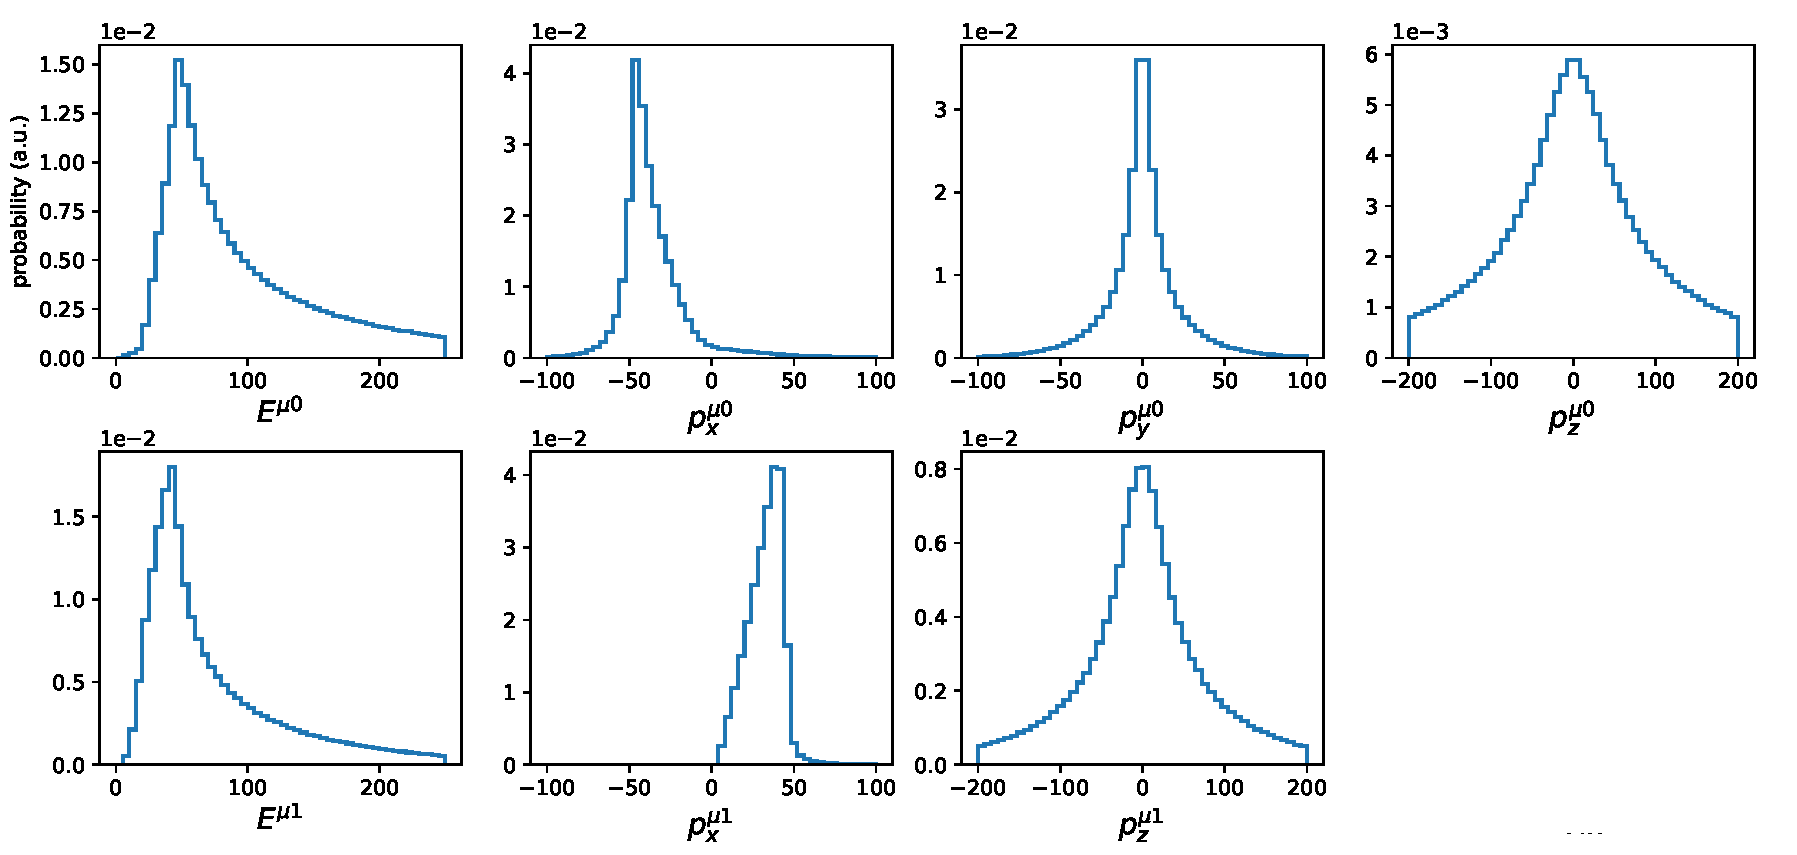
\includegraphics[width=\textwidth]{slides/pdfresizer.com-pdf-crop}
	\end{center}
\end{figure}
	
 \end{frame}



\begin{frame}{\underline{\secname}}
	
	\begin{center}
		\textbf{GANs to simulate Drell-Yan events in  ATLAS experiment}
	\end{center}
			\begin{itemize}			  \setlength\itemsep{0em}
\item
	
	The generator network consists of 7 fully connected layers with 64, 128, 256, 512, 256, 128, 7 neurons. Neurons in the inner layers are activated by leaky ReLU functions, while linear activation functions are used for the output layers. The input to the generator network consists of 7 ``noise'' floating-point numbers, sampled from a Gaussian distribution centered at 0 with unit variance. 
	
	\item

	The discriminator network consists of 9 hidden dense layers with 128, 128, 256, 256, 128, 64, 32, 16, and 8 neurons, activated by a leaky ReLU function. The last hidden layer is fully connected to a single-neuron output layer with sigmoid activation. In addition, a layer connected directly to the input layer returns the dilepton mass as part of the output.
	
\item

The combined network is trained adversarially for 40,000 epochs.

\item

All networks were implemented in {\tt KERAS}, using {\tt TensorFlow} as a back-end, The training was performed using Google TPU type (v2).	
	
				\end{itemize}

 \end{frame}

 
 
\begin{frame}{\underline{\secname}}
	
	
	\begin{center}
		\textbf{GANs to simulate Drell-Yan events in  ATLAS experiment}
	\end{center}	
	
	
\begin{figure}[H]
	\begin{center}
		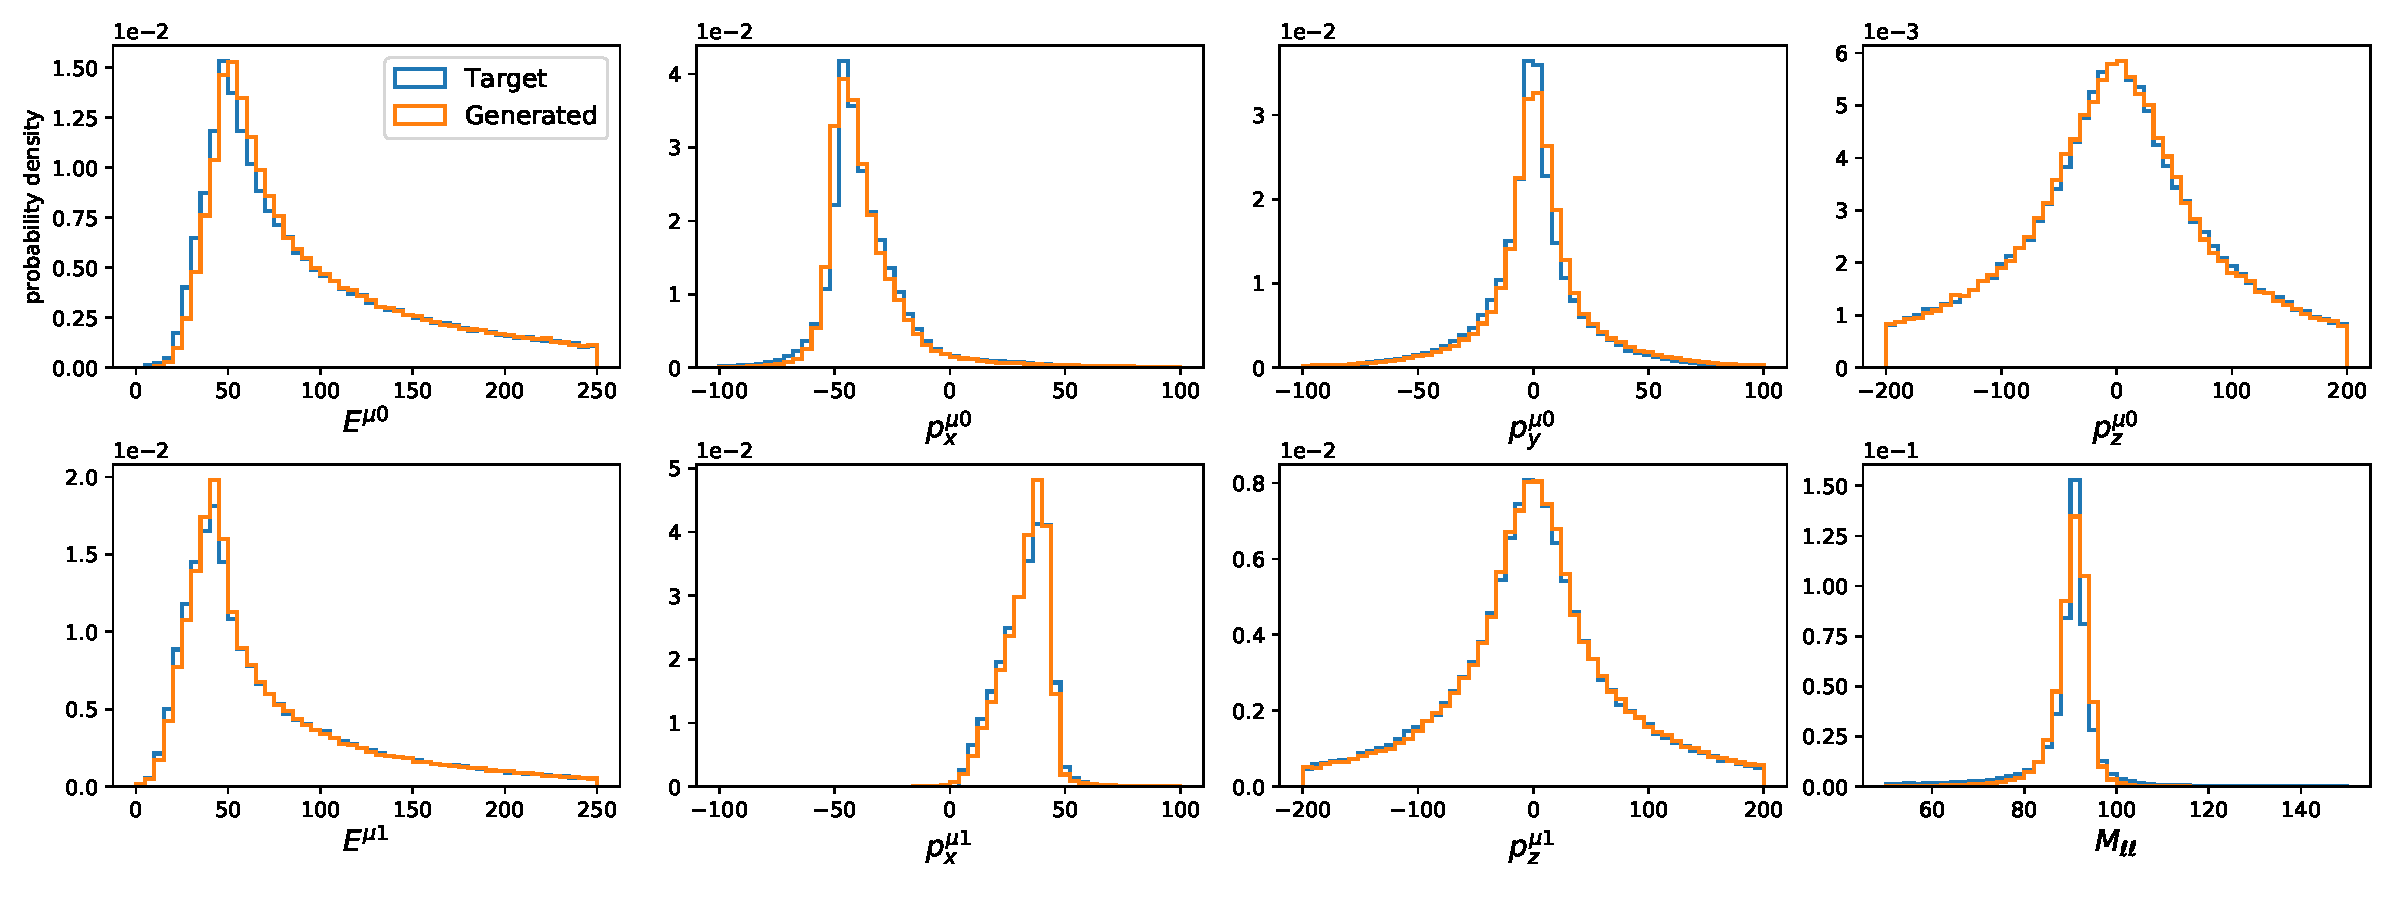
\includegraphics[width=\textwidth]{slides/trial9_epoch39700_minigantest_mllloss_final}
	\end{center}
\end{figure}
	
	


	
\end{frame}

\begin{frame}{\underline{\secname}}
	
	
	\begin{center}
		\textbf{Results}
	\end{center}	
	
			\begin{itemize}			  \setlength\itemsep{0em}
\item
	Results show that GANs can learn the multi-dimensional pdf of $\cal{O}$(7) features
\item
The GAN shows problems in learning distributions with sharp features such as edges
\item
 The Gan indicate a good performance but the reached precision is still insufficient to meet the precision requirements of an LHC data analysis.
			\end{itemize}

 	\begin{center}
		\textbf{Solutions}
	\end{center}
			\begin{itemize}			  \setlength\itemsep{0em}
\item Auxiliary GAN
\item reinforcement learning

\item  Conditional Hybrid GAN

			\end{itemize}
	
\end{frame}

% \section{Les trous noirs dans la théorie}

\subsection{Quelques mots sur la relativité générale}
%\begin{frame}{\underline{\secname} : {\small \subsecname}}
%
%
%\note{{\Huge cccccccccc}}
%\begin{block}{la relativité restrinte}
%	
%$$
%d s^{2}=-d t^{2}+d x^{2}+d y^{2}+d z^{2}
%$$	
%\end{block}
%  
%
%
%\begin{block}{le principe d’équivalence}
%\textit{"En tout point de l'espace-temps $\xi_{\mu}$, il est possible de choisir un système de coordonnées local $\xi_{\alpha}$ dans lequel les lois de la physique sont les mêmes que dans la relativité restreinte."}	
%	
%\end{block}
%
%
%\begin{block}{la relativité générale }
%la relativité générale = relativité restrinte +  le principe d’équivalence 
%$$
%d s^{2}=g_{\mu \nu} d x^{\mu} d x^{\nu}
%$$	
%	
%	\end{block}
%
%
%\end{frame}
\begin{frame}{\underline{\secname} : {\small \subsecname}}
\begin{block}{\Rightarrow Les équations d’Einstein}
\begin{itemize}
  \setlength\itemsep{0.5em}
\item Des équations dynamiques qui décrit comment la matière et l’énergie modifient la géométrie de l’espace-temps.
\item  L’équation la plus simple possible satisfaisant au principe d’équivalence.
\item Elle redonne l’équation de Newton dans une limite appropriée (la limite non relativiste).
\end{itemize}

\begin{columns}
	\begin{column}{0.5\linewidth}

\begin{eqnarray*}\label{einstien}
R_{\mu\nu}-\dfrac{1}{2}Rg_{\mu\nu}+g_{\mu\nu}\Lambda&=&8\pi GT_{\mu\nu} \\
\text{Courbure} &=&  \text{Matière énergie}
\end{eqnarray*}



\end{column}
\begin{column}{0.5\linewidth}

\begin{figure}
	\centering
	\includegraphics[width=0.9\linewidth,height=0.45\linewidth]{figures/space}
\end{figure}

\end{column}
\end{columns}

\end{block}


\end{frame}
\begin{frame}{\underline{\secname} : {\small \subsecname}}

Il est possible d'obtenir l'équation d'Einstein à partir du principe de moindre action: 
\begin{equation*}	
{\displaystyle S=\int \left[{\frac {1}{2\kappa }}(R-2\Lambda )+{\mathcal {L}}_{\mathrm {M} }\right]{\sqrt {-g}}\,\mathrm {d} ^{4}x}
\end{equation*}
\vspace{20pt}

\pause
\textbf{3 Solutions explicites avec degré maximal de symétrie des équations d'Einstein :}
\begin{itemize}
	  \setlength\itemsep{0.5em}
	\item Si $\Lambda = 0$ \Rightarrow la métrique de Minkowski $g=-dt^2+dx^2+dy^2+dz^2$.
	\item Si $\Lambda  > 0$ \Rightarrow la métrique de l'espace de-Sitter
	\item Si $\Lambda < 0$ \Rightarrow la métrique de l'espace anti-de-Sitter.
\end{itemize}


\end{frame}

\subsection{Les trous noirs dans la  relativité générale }

\begin{frame}{\underline{\secname} : {\small \subsecname}}
\begin{block}{Trou noir de Schwarzschild}
	
	
	\begin{itemize}
		\item Solution de l'équation d'Einstein dans le
		cas d'un champ gravitationnel statique à symétrie sphérique.
		\item La métrique est donnée par :
\begin{equation*}\label{schwarzchild}
d s^{2}=-\left(1-\frac{r_{S}}{r}\right) d t^{2}+\left(1-\frac{r_{S}}{r}\right)^{-1} d r^{2}+r^{2} d \Omega^{2}
\end{equation*}

\begin{equation*}r_{\mathrm{S}}=2 G M
\end{equation*}

			\item La métrique de Schwarzschild est singulière en  $ r = 2GM$ et $ r=0$
			

	\end{itemize}
	
\end{block}
\end{frame}



\begin{frame}{\underline{\secname} : {\small \subsecname}}
\begin{block}{Trou noir de Schwarzschild}
La courbure scalaire donne l’expression suivante :
$$R^{\mu\nu\alpha\beta}R_{\mu\nu\alpha\beta}=\dfrac{12r_{S}^{2}}{r^{6}}$$
\begin{itemize}
		  \setlength\itemsep{0.5em}
	\item $r = 0$ est une vraie singularité
\item $r=2GM$ est une singularité de coordonnées.(Horizon des évènements) \pause $\rightarrow$  \textbf{peut être effacée par un changement de coordonnées}
\end{itemize}

\vspace{20pt}

\begin{block}{	La métrique de Schwarzschild dans les coordonnées de Kruskal-Szekeres}
\begin{equation*}
ds^{2}=\dfrac{4r_{s}^{3}}{r}e^{-\frac{r}{r_{s}}}(du^{2}-dv^{2})+r^{2}(d\theta^{2}+sin^{2}\theta d\phi^{2})
\end{equation*}
\end{block}



\end{block}
\end{frame}

%
%\begin{frame}{\underline{\secname} : {\small \subsecname}}
%\begin{center}
%	\textbf{Les diagrammes conformes:}
%\end{center}
%	
%	  \begin{columns}
%\begin{column}{0.5\linewidth}
%
%Les diagrammes conformes constituent un bon moyen de faire correspondre des espace-temps complexes à un diagramme relativement simple. \\
%
%\vspace{20pt}
%\begin{center}\textbf{
%	l'infini $\infty$ $\rightarrow$ fini}
%\end{center}
%	
%\end{column}
%\begin{column}{0.5\linewidth}
%      \begin{figure}
%	\centering
%	\includegraphics[width=\linewidth]{figures/penrose_schw}
%	\caption{Diagramme de Penrose d'un trou noir de Schwarzschild}
%\end{figure}
%
%
%
%\end{column}
%\end{columns}
%\end{frame}


\begin{frame}{\underline{\secname} : {\small \subsecname}}

\begin{block}{Trou noir de Reissner Nordström}
	
	
	\begin{itemize}
		\item Solution de l'équation d'Einstein en présence de charge $Q$.
		$$R_{\mu\nu}-\dfrac{1}{2}g_{\mu\nu}R+g_{\mu\nu}\Lambda=8G\pi T_{\mu\nu}$$
		avec:
		$$T_{\mu\nu}=\dfrac{1}{4\pi}F_{\mu}^{\delta}F_{\nu\delta}-\dfrac{1}{4}g_{\mu\nu}F_{\alpha\beta}F^{\alpha\beta}$$
		\item La métrique est donnée par :
		$$ds^{2}=-(1-\dfrac{2M}{r}+\dfrac{Q^{2}}{r^{2}})dt^{2}+(1-\dfrac{2M}{r}+\dfrac{Q^{2}}{r^{2}})^{-1}dr^{2}-r^{2}d\theta^{2}-r^{2}sin^{2}(\theta)d\phi^{2}$$ 
	\end{itemize}
	
\end{block}
\end{frame}


\begin{frame}{\underline{\secname} : {\small \subsecname}}
\begin{block}{Trou noir de Reissner Nordström}

  \begin{columns}
	\begin{column}{0.5\linewidth}

\begin{itemize}
	\item 
	Si $G M^{2}<Q^{2}$ : Pas d'horizon des événements, 
	\item 
	Si $G M^{2}>Q^{2}$ : C'est une situation qui peut physiquement résulter d'un effondrement gravitationnel.\\
	Deux horizons $r_{+}$ et $r_{-}$
	\begin{equation*}
	r_{\pm}=G M \pm \sqrt{G^{2} M^{2}-G Q^{2} }
	\end{equation*}
	Et une singularité à $r = 0$
	\item 
	Si $G M^{2}=Q^{2}$ : Trou noir extrémal
\end{itemize}


\end{column}
\begin{column}{0.5\linewidth}
	

\begin{figure}[H]
	\begin{center}
		\includegraphics[width=\textwidth]{figures/plot.png}
	\end{center}
	\caption{La fonction $ f(r)=1-{2 G M}/{r}+{G Q^{2} }/{r^{2}}$ }
	\label{r-n}
\end{figure}
	
\end{column}
\end{columns}


\end{block}
\end{frame}



\begin{frame}{\underline{\secname} : {\small \subsecname}}
\begin{block}{Trou noir de Kerr}
	
	
	\begin{itemize}
		\item Solution exacte des équations d'Einstein permettant de décrire le comportement de l'espace-temps
		autour d'un trou noir en rotation $J\neq 0$ .
		
		\item La métrique est donnée par (avec les coordonnées de Boyer-Lindquist) :
		$$ds^{2}=-(1-\dfrac{2Mr}{\Sigma})dt^{2}+\dfrac{\Sigma}{\Delta}dr^{2}+\Sigma d\theta^{2}+\dfrac{Asin^{2}\theta}{\Sigma} d\phi^{2}-\dfrac{4Marsin^{2}\theta }{\Sigma} dt d\phi$$
		$$A=(r^{2}+a^{2})^{2}-\Delta a^{2}sin^{2}\theta ,\quad
		\Sigma =r^{2}+a^{2}cos^{2}\theta ,\quad
	     \Delta=r^{2}-2Mr+a^{2}  ,\quad
	     a=J / M
	     $$
		\item Si $M > a$  la métrique est singulière en:
		$$r_{\pm} = M \pm\sqrt{M^{2}-a^{2}}$$
		
	\end{itemize}
	
\end{block}
\end{frame}


%\begin{frame}{\underline{\secname} : {\small \subsecname}}
%\begin{block}{Trou noir de Kerr}
%	
%	\begin{columns}
%		\begin{column}{0.5\linewidth}
%\textbf{Ergosphère}:
%\vspace{20pt}
%
%C'est une région délimitée par la limite statique à l'extérieur, et par l'horizon externe à l'intérieur, dans laquelle rien ne peut rester immobile.\\
%\vspace{30pt}
%{\Rightarrow Il est possible d’extraire de l’énergie de rotation d’un trou noir de Kerr : \textbf{ Processus d’extraction d’énergie de Penrose }}
%		
%	\end{column}
%	\begin{column}{0.5\linewidth}
%
%
%\begin{figure}[H]
%	\begin{center}
%		\includegraphics[width=\textwidth]{figures/ergosphere.png}
%	\end{center}
%	\caption{Une vue de côté d'un trou noir de Kerr}
%	\label{kerr}
%\end{figure}
%
%\end{column}
%\end{columns}
%\end{block}
%\end{frame}

\begin{frame}{\underline{\secname} : {\small \subsecname}}

\begin{block}{Trou noir Kerr-Newman}
	
	
	\begin{itemize}
		\item  une solution de l'équation d'Einstein dans le cas d'un trou noir chargé et en rotation .
		
		\item Sa métrique est donnée par :
		$$ds^{2}=-\dfrac{\Delta}{\rho^{2}}(dt-asin^{2}\theta d\phi)^{2}+\dfrac{sin^{2}}{\rho^{2}}[(r^{2}+a^{2})d\phi-adt]^{2}+\dfrac{\rho^{2}}{\Delta}dr^{2}+\rho^{2}d\theta^{2}$$
		$$\Delta=r^{2}-2Mr+a^{2}+Q^{2} ,\quad	\rho^{2}=r^{2}+a^{2}cos^{2}\theta ,\quad a={J}/{M}$$
		
		
	\end{itemize}
\pause
\begin{itemize}
			  \setlength\itemsep{0em}
	\item  $Q=a=0$ \Rightarrow métrique de Schwarzschild
\item $a=0$ \Rightarrow métrique de Reissner Nordstrom
\item $ Q=0$ \Rightarrow métrique de Kerr
\item $M=Q=a=0$ \Rightarrow métrique d’un espace de Minkowski vide
\end{itemize}
\end{block}
\end{frame}


\begin{frame}{\underline{\secname} : {\small \subsecname}}
\begin{block}{The no-hair theorem}
	Les trous noirs sont totalement définis par un maximum de 3 paramètres. La masse, la charge et le moment angulaire.	$$M\,, Q\,, J $$
\end{block}

\begin{block}{L'insignifiance de la charge}
\begin{itemize}
				  \setlength\itemsep{0em}
	\item les forces électromagnétiques sont bien plus importantes que les forces gravitationnelles
\item le trou noir chargé va capturer toutes les particules de charge contraire disponibles et se neutraliser presque entièrement
\item la charge électrique des trous noirs peut être ignorée
\end{itemize}
	\end{block}



\vspace{10pt}
\pause
\begin{center}
	{\Large Les Trous Noirs Astrophysiques Sont Des Trous Noirs De Kerr}
\end{center}

\end{frame}
% \section{Les trous noirs en astrophysique}

\subsection{Les types de trous noirs}
\begin{frame}{\underline{\secname} : {\small \subsecname }}
  \begin{columns}
  	    \begin{column}{0.7\linewidth}

\begin{itemize}
	 \setlength\itemsep{0em}
	\item Trous noirs stellaires.
	 \begin{itemize}
	 	\item ~ 100m dans notre galaxie
	 	\item une masse entre 5 – 64 \(M_\odot\)
\item  le plus proche: HR 6819 situé \'{a} 1120 $A.L.$ %avec 5.0 \pm 0.4 \(M_\odot\)
	\end{itemize}
	\item Trous noirs intermédiaires.
\begin{itemize}
	\item peut se trouver dans les amas globulaire
	\item  masse entre 100 et 10 000 \(M_\odot\)
\end{itemize}

	\item Trous noirs supermassifs.
	 \begin{itemize}
\item  Le plus grand: TON618 avec  66 milliards \(M_\odot\)
\item Les vrais monstres !
\item au centre de toutes les galaxies spirales et elliptiques

	\end{itemize}

%	\item Trous noirs primordiaux. 
%	 \begin{itemize}
%		\item seulement théorique, jamais observé
%		\item Peut avoir été créé peu après le Big Bang
%		\item Peut être créé dans les accélérateurs de particules
%	\end{itemize}
\end{itemize} 

 \end{column}
\begin{column}{0.3\linewidth}
      \begin{figure}
	\centering
\includegraphics[width=\linewidth]{figures/Black_hole_-_Messier_87_crop_max_res.jpg}
	\caption{Image du trou noir supermassif M87*}
\end{figure}
\end{column}
\end{columns}

\end{frame}


{
%	\setbeamercolor{background canvas}{bg=black}

\subsection{La formation des Trous Noirs}
\begin{frame}{\underline{\secname} : {\small \subsecname}}

%\usebackgroundtemplate{\includegraphics[width=\paperwidth]{figures/formation.png}}


\begin{tikzpicture}
\node[anchor=south west,inner sep=0] (image) at (0,0) {\includegraphics[width=0.9\paperwidth,height=0.7\paperheight]{figures/use5128.png}};
\framenode[15pt]{image} % opt. arg. is fade radius; mand. arg. is node name to frame
\end{tikzpicture}
%\includegraphics[width=\paperwidth,height=\paperheight]{figures/formation.png}


\begin{itemize}
		 \setlength\itemsep{0em}
\item 1.4 \(M_\odot\)  limite de Chandrasekhar : Max d’une naine blanche

\item 3 \(M_\odot\) limite de Tolman-Oppenheimer-Volkoff : Max d’une étoile à neutron
\end{itemize}




\end{frame}

}

\begin{frame}{\underline{\secname} : {\small \subsecname}}

\begin{center}
	\textbf{La formation des Trous Noirs intermédiaires et supermassifs}
\end{center}
 \begin{columns}
	
	\begin{column}{0.5\linewidth}
				      \begin{figure}
			\includegraphics[width=\linewidth,height=140pt]{figures/une-trois-trous-noirs-collision-1024x535}
			\caption{Collisions de trous noirs}
			
			
		\end{figure}
	\end{column}
	\begin{column}{0.5\linewidth}
		      \begin{figure}
	\includegraphics[width=\linewidth,height=140pt]{figures/bhbinary}
	\caption{Accrétion de la matière}
	
	
\end{figure}
	\end{column}
\end{columns}
\end{frame}

\subsection{La détection des trous noirs}
\begin{frame}{\underline{\secname} :Comment détecter un trou noir ?}

\begin{center}
	\textbf{Comment détecter un trou noir ?}
\end{center}

 \begin{columns}

	\begin{column}{0.6\linewidth}	
	\begin{itemize}  \setlength\itemsep{0.5em}
		\item  Les systèmes binaires
%		\item  Les rayons gamma
%
%\begin{itemize}
%	\item 			 L’explosion d’une étoile massive en supernova
%\end{itemize}
%
%		\item  La présence de jets
%
%\begin{itemize}
%	\item 			Disque d’accrétion $\rightarrow$ Rayonnement $X$
%\end{itemize}
%
%		\item  La détection des ondes gravitationnelles


	\item 		détecteurs interférométriques d’ondes gravitationnelles 	(LIGO $\&$ Virgo)
	\item 			Disque d’accrétion $\rightarrow$ Rayonnement $X$

	\end{itemize}	
		
	\end{column}
	\begin{column}{0.4\linewidth}
		
		\begin{block}
	
 %	\includegraphics[width=\paperwidth,height=\paperheight]{figures/bhbinary_xmm_960.jpg}
	
	% \includegraphics[width=\paperwidth,height=\paperheight]{figures/jets.png}
\begin{center}

		      \begin{figure}
		      	\includegraphics[width=\linewidth,height=120pt]{figures/ligo}
		   	\caption{le détecteur LIGO}

		
	\end{figure}
\end{center}
	
	
			
		\end{block}	
	\end{column}
\end{columns}
 
\end{frame}
% 
% 

\section{La thermodynamique des trous noirs}
\begin{frame}{\underline{\secname} }

%\begin{block}{La thermodynamique}
%Science qui sait comprendre des aspects essentiels des systèmes macroscopiques sans connaitre leurs aspects microscopiques.
%\end{block}


\begin{block}{L’expérience de pensée de Wheeler (1970)}
Que se passe-t-il si nous jetons une tasse de thé dans un trou noir?
\pause
\begin{enumerate}
		\item Le thé est chaud - il a une entropie $(S_{the} > 0)$
		\pause
	\item Le trou noir absorbe tout et n'a pas de structure interne $(S_{TN} = 0)$
\pause
	\item $(S_{total} = 0)$  $\rightarrow$ violation du deuxième principe de la thermodynamique 
\end{enumerate}	
	
\end{block}

\pause
\textbf{Bekenstein}: Le thé a une masse  \Rightarrow il va augmenter la masse du trou noir \Rightarrow l'aire de l'horizon doit augmenter + Théorème des aires de Hawking

\pause

\begin{center}
	%suggéra donc que l’entropie généralisé ne peut que croı̂tre.
{\Large $A$ (l'aire de l'horizon)   $\Leftrightarrow$     $S$ (l’entropie)}
\end{center}


%The total area of a closed system never decreases.


\end{frame}

\subsection{La  température  et l’entropie }
\begin{frame}{\underline{\secname} : {\small \subsecname}}
\begin{center}
\textbf{	Débat entre Hawking et Beckenstein }
	
\end{center}
{\color{red}Hawking}: l'analogie entre le théorème d'aire et la $2^{\`{e}me}$ loi de la thermodynamique n'est qu'une question de coïncidence.

\vspace{10pt}
{\color{red}Beckenstein}: Je n'en suis pas convaincu. Nulle part dans la nature, la deuxième loi de la thermodynamique n'est violée. Pourquoi les trous noirs seraient-ils une exception ?
\vspace{10pt}

{\color{red}Wheeler} (Le directeur de thèse de Beckenstein) a dit à Beckenstein: Votre idée est tellement folle qu'elle pourrait bien être vraie.
\vspace{10pt}

{\color{red}Hawking}: si un trou noir a une entropie, il doit avoir une température, et s'il a une température, il doit irradier comme un corps noir. Mais si rien ne peut s'échapper d'un trou noir, comment peut-il rayonner ?


\end{frame}

\begin{frame}{\underline{\secname} : {\small \subsecname}}


\begin{center}
	\textbf{1974: fin du débat et découverte du rayonnement Hawking}
\end{center}

\begin{columns}
	\begin{column}{0.6\linewidth}

\begin{itemize}
			 \setlength\itemsep{0.5em}
	\item Les effets quantiques près de l'horizon des événements permettent aux particules de s'échapper du potentiel gravitationnel.

\item Le trou noir perd de l'énergie (et de la masse) 

\item Les trous noirs rayonnent comme un corps noir avec une température
\end{itemize}

\begin{center}
	%suggéra donc que l’entropie généralisé ne peut que croı̂tre.
\textbf{	{\large $\kappa$ (la gravité de surface)   $\Leftrightarrow$     $T$ (la température)}}
\end{center}

\end{column}
\begin{column}{0.4\linewidth}
	
      \begin{figure}
	\centering
	\includegraphics[width=1.2\linewidth,height=170pt]{figures/hawking}
\end{figure}

\end{column}
\end{columns}

\end{frame}
\begin{frame}{\underline{\secname} : {\small \subsecname}}

\begin{block}{l’entropie de Trou Noir}
L'entropie du trou noir est liée à la surface de l'horizon par la relation,

$$S=\frac{k_{B} c^{3}}{4 G \hbar} A$$
\end{block}

\begin{block}{la température de Trou Noir}
La tempurature du trou noir (formule de Bekenstein-Hawking)

$$T_{h}=\frac{\hbar}{2 \pi k_{b} c} \kappa$$
\end{block}

\pause
\textbf{Les formules contient toutes les constantes fondamentales:}\\

%\begin{eqnarray*}\text{
%la constante de Planck &$\hbar$&\\
%la constante de Boltzmann &$k_b$&\\
%la vitesse de la lumière &$c$&\\
%la constante de Newton &$G$&\\
%}
%\end{eqnarray*}  \Rightarrow $$ \text{La théorie d’unification} $$

	$$ \hbar, k_b, c, G,\Rightarrow \text{La théorie d’unification}$$
\end{frame}

%\begin{frame}{\underline{\secname} : {\small \subsecname}}
%\begin{block}{Évaporation des trous noirs}
%Grâce au résultat de Hawking on peut calculer La luminosité et La durée de vie :
%
%\vspace{20pt}
%\begin{columns}
%	\begin{column}{0.5\linewidth}
%\textbf{la luminosité du rayonnement de Hawking }
%\begin{equation*}
%L=A \sigma T^{4}=\frac{\hbar c^{2}}{3840 \pi a^{2}}=\frac{\hbar c^{6}}{15639 \pi G^{2} M^{2}}
%\end{equation*}
%\end{column}
%\begin{column}{0.5\linewidth}
%\textbf{La durée de vie d'un trou noir}
%
%\begin{equation*}
%\tau=\int_{0}^{\tau} \mathrm{d} t=-\frac{15360 \pi G^{2}}{h c^{4}} \int_{0}^{M} M^{2} \mathrm{d} M
%\end{equation*}
%
%\end{column}
%\end{columns}
%
%\end{block}
%\vspace{20pt}
%\pause
%\begin{center}
%	{\Large $\Rightarrow \tau \cong 0 \quad  L \cong 0 $ }
%\end{center}
%
%\end{frame}


\subsection{Les $\rom{4}$ lois de la thermodynamique}
\begin{frame}{\underline{\secname} : {\small \subsecname}}

\begin{block}{Principe Zéro}
	
	La gravité de surface $\kappa$ d'un trou noir stationnaire est constante sur toute la surface de l'horizon	
\end{block}
\begin{block}{Premier Principe}
	$$dM=\dfrac{k}{8\pi}\delta A+\Omega_{h}\delta J+\Phi_{h}\delta Q$$
	la variation de la masse entraîne une variation de l'énergie cinétique angulaire $\Omega_{h}\delta J$, une variation de l'énergie potentielle électrique $\Phi_{h}\delta Q$ et une variation d'énergie de rayonnement $\dfrac{k}{8\pi}\delta A$.
\end{block}

\end{frame}

\begin{frame}{\underline{\secname} : {\small \subsecname}}
\begin{block}{Dexième Principe}
 L'aire A de l'horizon des événements de chaque trou noir ne peut pas décroître $\delta A\geq 0$. 

\vspace{10pt}

\textbf{le deuxième principe généralisée de la thermodynamique :} L'entropie commune à l'extérieur du trou noir plus l'entropie du trou noir ne diminue jamais $S=S_{T N}+S_{\text{ext}}$
$$
\delta S \geq 0
$$


\end{block}
\begin{block}{Troisième Principe}
 On ne peut pas atteindre $\kappa = 0$ par aucun processus.
\end{block}

\end{frame}


\subsection{L’analogie avec la thermodynamique standard}


\begin{frame}{\underline{\secname} : {\small \subsecname}}
\begin{center}
	\textbf{Où est le terme $P \delta V$ dans le premier principe?}
		$$dM=\dfrac{k}{8\pi}\delta A+\Omega_{h}\delta J+\Phi_{h}\delta Q$$
\end{center}
\pause
Solution : 
\begin{itemize}		 \setlength\itemsep{0.5em}
	\item traiter $\Lambda$ comme une pression thermodynamique \item
Masse $M$ interprétée comme une enthalpie plutôt qu'une énergie \item
nous pouvons l'utiliser pour calculer le volume thermodynamique associé au trou noir $$V= \left(\frac{\partial M}{\partial P} \right)_S$$
\end{itemize}
\pause 
le premier principe devient la formule suivante:
 %TODO 
\begin{center}
	$$dM=\dfrac{k}{8\pi}\delta A+\Omega_{h}\delta J+\Phi_{h}\delta Q +P \delta V$$
 
\end{center}

%The PV term in this equation can be though of as the contribution to the mass-energy of the
%black hole due the negative energy density of the vacuum, ǫ = −P, associated with a positive
%cosmological constant. If the black hole has volume V then it contains energy ǫV = −PV
%and so the total energy is U = M − PV.

\end{frame}




\begin{frame}{\underline{\secname} : {\small \subsecname}}
\begin{block}{ L’analogie avec la thermodynamique standard }
		
	\begin{eqnarray*}
	\textrm{Enthalpie}\quad  H &\leftrightarrow&  M\quad  \textrm{Masse}   \nonumber\\
	\textrm{Température}\quad  T &\leftrightarrow&  \frac{\kappa}{2\pi} \quad  \textrm{Gravité de surface}   \nonumber\\
	\textrm{Entropie}\quad  S &\leftrightarrow&  \frac{A}{4 } \quad  \textrm{l'aire de l'horizon}   \nonumber\\
	\textrm{Pression}\quad  P &\leftrightarrow&  -\frac{\Lambda}{8\pi} \quad  \textrm{Constante cosmologique}   \nonumber\\
	\textrm{Volume}\quad  V &\leftrightarrow&  \left(\frac{\partial M}{\partial P} \right)_S \quad  \textrm{Volume thermodynamique}   \nonumber\\
	\end{eqnarray*}

	
\end{block}
\end{frame}

\begin{frame}{\underline{\secname} : {\small \subsecname}}
% Une fois le volume thermodynamique connu 
\begin{block}{La stabilité thermodynamique}

\begin{itemize}
	\item  L'équation d'état du "fluide" 
\begin{equation*}
P=P(V,T,J,Q)
\end{equation*}
\item La thermodynamique d'équilibre est régie par l'énergie libre de Gibbs: {\color{green}\textbf état équilibre correspond au minimum global de G}
\begin{equation*}
G=M-TS=G(P,T,J, Q)\,. 
\end{equation*}
\item La stabilité thermodynamique locale est caractérisée par {\color{green}\textbf la positivité de la chaleur spécifique} à pression constante (et $Q$ où $J$ fixe) 
\begin{equation*}
C_P\equiv C_{P,J,Q}=T\left(\frac{\partial S}{\partial T}\right)_{P,J,Q}
\end{equation*}	

\end{itemize}	
	\end{block}
	

\end{frame}

% \section{Les transitions de phase des trous noirs}

\begin{frame}{\underline{\secname} : Espace Asymptotiquement Plat}
\begin{block}{Trou noir de Schwarzschild :}
	
	\begin{columns}
		\begin{column}{0.5\linewidth}
		
	\begin{eqnarray*}
	T&=&\frac{1}{4\pi r_s}\,,\quad
	S=\frac{A}{4}=\pi r_s^2\,,\nonumber\\ G&=&\frac{r_s}{4}=\frac{1}{16\pi T}\,,\quad
	C_P=-2 \pi r_s^2<0\,,
	\end{eqnarray*}	
	\pause		
	
\begin{center}
	\textbf{Un trou noir de Schwarzschild est thermodynamiquement instable 	}
\end{center}

		\end{column}
		\begin{column}{0.5\linewidth}
			\begin{figure}[H]
				\begin{center}
					
					\includegraphics[width=\textwidth,height=140pt]{figures/GscF}
					
					\caption{$G(T)$ pour le trou noir de Schwarzschild}
				\end{center}
			\end{figure}
			
			
		\end{column}
	\end{columns}
\end{block}
\end{frame}


\begin{frame}{\underline{\secname} : Espace Asymptotiquement Plat}
\begin{block}{Trou noir de Reissner Nordstrom :}
	
	\begin{columns}
		\begin{column}{0.5\linewidth}
				\begin{eqnarray*}
		S&=& \pi r_s^2\,,\quad
		T = \frac{r_+^2-Q^2}{4\pi r_+^3}\,,\nonumber\\
		G&=&\frac{r_+^2+3Q^2}{4r_+}\,,\quad C_P=2\pi r_+^2\frac{r_+^2-Q^2}{3Q^2-r_+^2}\,,
			\end{eqnarray*}	
			
$C_p$ est positive  pour $\sqrt{3}|Q|> r_+>|Q|\,,$
	\pause		

\begin{center}
	\textbf{les petits trous noirs presque extrémaux fortement chargés sont thermodynamiquement préférée et stable}
\end{center}			
			
		\end{column}
		\begin{column}{0.5\linewidth}
			\begin{figure}[H]
				\begin{center}
					\includegraphics[width=\textwidth,height=140pt]{figures/Gkerrflat}
					
					\caption{$G(T)$ pour le trou noir de de Reissner Nordstrom}
				\end{center}
			\end{figure}
			
			
		\end{column}
	\end{columns}
\end{block}
\end{frame}



\begin{frame}{\underline{\secname} : Espace Asymptotiquement Plat}
\begin{block}{Trou noir de Kerr :}
	
	\begin{columns}
		\begin{column}{0.6\linewidth}
\begin{eqnarray*}
T&=&\frac{1}{2\pi}\bigg[\frac{r_+}{a^2+r_+^2}-\frac{1}{2r_+}\bigg]\,,\quad 
S=\pi(a^2+r_+^2)\,,\nonumber\\
H&=&\frac{r_+^2+a^2}{2r_+}\,,\quad  G=\frac{3a^2+r_+^2}{4r_+} \,,\nonumber\\
C_P&=&\frac{2\pi(r_+^2-a^2)(r_+^2+a^2)^2}{3a^4+6r_+^2a^2-r_+^4}
\end{eqnarray*}
$C_p$ est positive pour $\sqrt{3+2\sqrt{3}}|a|>r_+>|a|$

\pause
\begin{center}
	\textbf{les petits petits trous noirs à rotation rapide presque extrêmes sont thermodynamiquement préférée et stable}
\end{center}
		\end{column}
		\begin{column}{0.4\linewidth}
			\begin{figure}[H]
				\begin{center}
					\includegraphics[width=\textwidth,height=140pt]{figures/figure1}
				\end{center}
			\end{figure}
			
			
		\end{column}
	\end{columns}
\end{block}
\end{frame}







\begin{frame}{\underline{\secname} : Espace Asymptotiquement AdS}
\begin{block}{Trou noir de Schwarzschild AdS :}
les grandeurs thermodynamiques :
\begin{columns}
	\begin{column}{0.5\linewidth}
		la pression
$$P=-\dfrac{\Lambda}{8 \pi}=\dfrac{3}{8 \pi l^2}$$
La variable conjuguée à la pression
$$V= \left(\frac{\partial M}{\partial P} \right)_S=\frac{4}{3}\pi r_s^3$$
\pause
$\Rightarrow$ C’est le volume géométrique d’une sphère de rayon $r_s$ a 3 dimention
\pause
	\end{column}
\begin{column}{0.5\linewidth}
 			
 \begin{eqnarray*}
T&=&\frac{1}{4\pi r_s l^2}(l^2+3r_s^2)\,,\nonumber\\
S&=&\pi r_s^2\,,\quad 
H=\frac{r_s}{2}\Bigl(1+\frac{r_s^2}{l^2}\Bigr)\,,\nonumber\\ G&=&\frac{r_s}{4}\Bigl(1-\frac{r_s^2}{l^2}\Bigr)\,,\quad
C_P=2\pi r_s^2\frac{3r_s^2+l^2}{3r_s^2-l^2}\,,
 \end{eqnarray*}
	\end{column}
\end{columns}
\end{block}

\end{frame}

\begin{frame}{\underline{\secname} : Espace Asymptotiquement AdS}


\begin{center}
	\textbf{La stabilité et la chaleur spécifique}
\end{center}

\begin{columns}
	\begin{column}{0.5\linewidth}
La température minimale
$$\dfrac{\partial T}{\partial r_{+}}=0 \Leftrightarrow T_{min}=\dfrac{\sqrt{3}}{2\pi l}, \pause \Rightarrow$$
	\begin{itemize}
		\item $T < T_{min} $ la chaleur spécifique est négative, dans ce cas le système thermodynamique est instable .
		\item $T > T_{min} $ la chaleur spécifique est positive, donc c’est la région stable.
		
	\end{itemize}

		
\end{column}
\begin{column}{0.5\linewidth}
	
			\begin{figure}
		\begin{center}
			\includegraphics[width=\textwidth,height=140pt]{figures/path3285.png}
		\end{center}
	\end{figure}
			
\end{column}
\end{columns}

\end{frame}

\begin{frame}[t]{\underline{\secname} : Espace Asymptotiquement AdS}
\begin{center}
	\textbf{Transition de phase Hawking–Page:}
\end{center}

\begin{columns}
	\begin{column}{0.5\linewidth}
		 La transition de phase 
		$$G=0 \Leftrightarrow T_{HP}=\dfrac{1}{\pi l}.$$
	\begin{itemize} \setlength\itemsep{0em}
		\item  Pour $T < T_{min}$ , seulement la phase "rayonnement thermique pure" qui existe.
		\item  Pour $T_{min} < T < T_{HP}$ la phase "rayonnement thermique" est plus stable
		\item  Pour $T > T_{HP}$ la phase "large trou noir" c'est la plus stable
		
	\end{itemize}
		
		
	\end{column}
	\begin{column}{0.5\linewidth}
		\begin{figure}
			\begin{center}
				\includegraphics[width=\textwidth,height=140pt]{figures/g512.png}
				\label{Fig:Gschads}
			\end{center}
		\end{figure}
		
		
	\end{column}
\end{columns}
\end{frame}

\begin{frame}{\underline{\secname} : Espace Asymptotiquement AdS}

\begin{columns}
	\begin{column}{0.5\linewidth}
La ligne de coexistence des deux phases : rayonnement thermique/large trou noir s'écrit comme suit :
$$
P_{HP} =\frac{3 \pi}{8} T^2_{HP} 
$$
	\end{column}
\begin{column}{0.5\linewidth}
\begin{figure}
	\begin{center}
		\includegraphics[width=\textwidth,height=140pt]{figures/HPtransition}
	\end{center}
\end{figure}


\end{column}
\end{columns}
\end{frame}

%%%%%%%%%%%%%%%%%%%%%%%%%%%%%%%%%%%%%%%%%%%%


\begin{frame}{\underline{\secname} : Espace Asymptotiquement AdS}
\begin{block}{Trou noir de Reissner Nordstrom AdS :}
	les grandeurs thermodynamiques :
	
	\begin{eqnarray*}
T&=&\frac{1}{4\pi r_+^3 l^2}\Bigl(l^2(r_+^2-Q^2)+3r_+^4\Bigr)\,,\quad S=\pi r_+^2\,,\nonumber\\
V&=&\frac{4}{3}\pi r_+^3\,,\quad \Phi=\frac{Q}{r_+}\,,\quad 
G=\frac{l^2r_+^2-r_+^4+3Q^2l^2}{4l^2r_+}\,,\nonumber\\
C_P&=&2\pi r_+^2\frac{3r_+^4+l^2r_+^2-Q^2l^2}{3r_+^4-l^2r_+^2+3Q^2l^2}\,.\quad M= \frac{1}{2}\left(r_{+}-\frac{Q^{2}}{r_{+}}+\frac{8 \pi}{3} r_{+}^{3} P\right)
	\end{eqnarray*}


	
\end{block}

\end{frame}



\begin{frame}{\underline{\secname} : Espace Asymptotiquement AdS}

	\begin{columns}
		\begin{column}{0.6\linewidth}
\begin{itemize} \setlength\itemsep{0em}
	\item On peut écrire la pression comme:
	
	\begin{equation*}
	P=\frac{T}{\nu}-\frac{1}{2\pi \nu^2}+\frac{2Q^2}{\pi \nu^4}  \quad \text{avec: } \nu=2l_{p}^{2}r_{+}
	\end{equation*}
	\pause[2]
	$\Rightarrow$ Un équation d'état de \textbf{Van der Waals}:


\pause[3]
	\item	Le point critique:	
	\begin{equation*}
	\frac{\partial P}{\partial \nu}=0 \quad \text { et } \quad \frac{\partial^{2} P}{\partial \nu^{2}}=0
	\end{equation*}
			$$
			T_c=\frac{\sqrt{6}}{18\pi Q}\,,\quad \nonumber v_c=2\sqrt{6} Q\,,\quad \nonumber P_c=\frac{1}{96\pi Q^2}\,, 
			$$	
			
	\pause[4]				
\item la relation $\rho_c=P_c v_c/T_c=3/8$ est identique au cas de Van der Waals. 			
			
\end{itemize}
		\end{column}
		\begin{column}{0.4\linewidth}
			\pause[2]
			\begin{figure}[H]
				\begin{center}
			 
						\includegraphics[height=140pt,width=\textwidth]{figures/rP.pdf}
					
					\caption{Equation d'état d'un trou noir chargé AdS.}
				\end{center}
			\end{figure}
			
		\end{column}
	\end{columns}

\end{frame}


\begin{frame}{\underline{\secname} : Espace Asymptotiquement AdS}
\begin{center}
		\textbf{Transition de phase (SBH/LBH):}
\end{center}
\begin{columns}
	\begin{column}{0.5\linewidth}
		\begin{itemize} \setlength\itemsep{0.5em}
			\item  $P < P_c$ l’allure de $G$ montre une transition de phase du premier ordre
			\item  $P = P_c$ la transition de phase est de deuxième ordre 
			\item  $P > P_c$ pas de transition de phase
		\end{itemize}	
	\end{column}
	\begin{column}{0.5\linewidth}
\begin{figure}[H]
	\begin{center}

			\includegraphics[width=\textwidth,height=0.7\linewidth]{figures/GrnAdS.eps}
		
		\caption{ $G(T)$ d'un trou noir de RN-AdS.}
	\end{center}
\end{figure}
		
		
	\end{column}
\end{columns}

\end{frame}

%%%%%%%%%%%%%%%%%%%%%%%%%%%%%%



\begin{frame}{\underline{\secname} : Espace Asymptotiquement AdS}
\begin{block}{Trou noir de Kerr AdS :}
	les grandeurs thermodynamiques :
\begin{eqnarray*}
T&=&\frac{r_{+}}{4\pi(r_{+}^{2}+a^{2})}
\left(1+\frac{a^{2}}{l^{2}}+3\frac{r_{+}^{2}}{l^{2}}-\frac{a^{2}}{r_{+}^{2}}\right),\\
S&=&\frac{\pi (r_{+}^{2}+a^{2})}{\Xi},\quad 
\\
G&=&\frac{a^4 \left(r_{+}^2-l^{2}\right)+a^2\left(3l^{4}
	+2l^{2}r_{+}^2+3r_{+}^4\right)+l^{2} r_{+}^2
	\left(l^{2}-r_{+}^2\right)}{4 r_{+}\left(a^2-l^{2}\right)^2}.\quad 
\\
C_P &=& \frac{2 \pi l^4  \left(a^2+r_{+}^2\right)^2 \left(-a^2 l^2+\left(a^2+l^2\right) r_{+}^2
	+3 r_{+}^4\right)}{(l^2 -a^2) X},
\end{eqnarray*}
\end{block}
\end{frame}


%
%\begin{frame}{\underline{\secname} : Espace Asymptotiquement AdS}
%	
%	\begin{columns}
%		\begin{column}{0.5\linewidth}
% $$C_p(r)   \Rightarrow  C_p(p,s) $$
%
%Avec $p$ et $s$ les paramètres normalisés
%\begin{equation*}
%		p \equiv \frac{|a|}{r_{+}}, ~\mbox{and}~~ s \equiv \frac{l}{r_{+}}.
%\end{equation*}
%\begin{itemize}
%	\item 		Dans la région $\rom{1}$, $C_{P} <0$
%	\item	Dans la région $\rom{2}$,$C_{P} >0$
%	\item		Dans la région $\rom{3}$, il n'y a pas de solution physique parce que $|a| > l$.			
%\end{itemize}
%		\end{column}
%		\begin{column}{0.5\linewidth}
%		\begin{figure}[H]
%			\noindent\hfil\includegraphics[width=\linewidth,height=0.7\linewidth]{figures/figure14.eps}
%			\caption{Diagramme de phase des trous noirs de Kerr-AdS.}
%			\label{fig:heat_capacity_AdS}
%		\end{figure}
%
%			
%		\end{column}
%	\end{columns}
%
%\end{frame}




\begin{frame}{\underline{\secname} : Espace Asymptotiquement AdS}
	 Dans la limite du petit $J$ on obtient une valeur approximative de point critique \footnote{Shao-Wen Wei, Peng Cheng et Yu-Xiao Liu. “Analytical and exact critical phenomena ofd-dimensional singly spinning Kerr-AdS black holes”}:
	\begin{columns}
		\begin{column}{0.5\linewidth}
 	
			$$P_c \simeq  0.002857 \cdot J^{-1}$$
			$$V_c \simeq 6.047357 \cdot J^{1/2},$$
			$$T_c \simeq 115.796503 \sqrt[3]{J},$$

	\pause[3]		
	
	\begin{center}
		\textbf{Les résultats sont les mêmes que ceux du trou noir RN-AdS}	\\	
		{\color{green}Transition de phase (SBH/LBH)	}
	\end{center}

		\end{column}
		\begin{column}{0.5\linewidth}
			\pause[2]
	\begin{figure}[H]
		\begin{center}
			%	\rotatebox{-90}{
			\includegraphics[width=\textwidth,height=120pt]{figures/KerrGT_3b.eps}
			%	}
			\caption{ $G(T)$ d'un trou noir de Kerr-AdS.} \label{Fig:KKGT} 
		\end{center}
	\end{figure} 	
			
		\end{column}
	\end{columns}
\end{frame}



% \chaptertoc{Conclusion Générale}
\thispagestyle{empty}





\section{Why this thesis}

\begin{frame}{\underline{\secname}}
	

	\begin{center}
		\textbf{Why this thesis}
	\end{center}
				\begin{itemize}			  \setlength\itemsep{0em}
\item
I’ve enjoyed my academic work so far, but I really feel I’ve got more to offer as an independent researcher. I’m also passionate about this subject and don’t feel enough attention has been paid to the questions I’m looking to address (appling deep learning to data analysis in lhc big data) .
\item

	
	This thesis combine two of my favorite field: experimental particle physics \& machine learning,
\item
	
I think CEA can help me with these ambitions since it has a strong ATLAS group with access to formidable computational resources.	
\end{itemize}

	\begin{center}
		\textbf{}
	\end{center}
	after complete the PhD I plan to pursue a postdoc likely in the area of unsupervised machine learning in data analysis of the ATLAS experiment.
	
\end{frame}



%========================
% thanks
%========================


{
	\usebackgroundtemplate{ \centering \includegraphics[height=\paperheight,width=\paperwidth]{figures/ALICE-pic.pdf}}%
\begin{frame}\frametitle{{\color{white}Finally...}}


\centering

{\vspace{17em} \Huge {\color{white}	\textbf{Thanks For Your Attention !!}\\}}
\end{frame}

}


%=================================================
% end presentation
%=================================================
\end{document}
